%%%%%%%%%%%%%%%%%%%%%%%%%%%%%% -*- Mode: Latex -*- %%%%%%%%%%%%%%%%%%%%%%%%%%%%
%% proposal.tex -- 
%% Author          : Robert Brewer
%% Created On      : Tue Jan 10 11:53:15 1995
%% Last Modified By: Robert Brewer
%% Last Modified On: Mon Jan 31 16:48:09 2000
%% Status          : Unknown
%% RCS: $Id: proposal.tex,v 1.3 1999/02/02 04:17:26 rbrewer Exp $
%%%%%%%%%%%%%%%%%%%%%%%%%%%%%%%%%%%%%%%%%%%%%%%%%%%%%%%%%%%%%%%%%%%%%%%%%%%%%%%
%%   Copyright (C) 1998 Robert Brewer
%%%%%%%%%%%%%%%%%%%%%%%%%%%%%%%%%%%%%%%%%%%%%%%%%%%%%%%%%%%%%%%%%%%%%%%%%%%%%%%
%% 
%% For building official version w/o titlepage or abstract
\documentclass [11pt] {article}

%% New LaTeX2e graphics support
\usepackage[final]{graphicx}
%% Support for decent URL output
\usepackage{url}
%% Switch to Times Postscript font
\usepackage{times}

%% Make the margins sane, must be in preamble to work properly
\setlength{\oddsidemargin}{0in}
\setlength{\textwidth}{6.5in}
\setlength{\textheight}{8.6in}
\setlength{\topmargin}{0in}
\setlength{\headheight}{0in}
\setlength{\headsep}{0in}
\setlength{\topskip}{1pt}
\setlength{\footskip}{0.75in}

\title{Aspect Technology Fund Grant Proposal:\\Adaptive Spam Detection and
Removal Tool}
\author{Robert S. Brewer\\Collaborative Software Development Lab\\University of
Hawaii at Manoa}

\date{February 1, 2000}

\begin{document}

%% For building CSDL internal version with titlepage and abstract
%\maketitle

%\begin{abstract}
%  Spam tool abstract to be written...
%\end{abstract}

%%%%%%%%%%%%%%%%%%%%%%%%%%%%%% -*- Mode: Latex -*- %%%%%%%%%%%%%%%%%%%%%%%%%%%%
%% project-description.tex -- 
%% Author          : Robert Brewer
%% Created On      : Wed Jan 27 16:28:11 1999
%% Last Modified By: Robert Brewer
%% Last Modified On: Mon Feb  1 14:16:44 1999
%% RCS: $Id: project-description.tex,v 1.5 1999/02/02 04:02:05 rbrewer Exp $
%%%%%%%%%%%%%%%%%%%%%%%%%%%%%%%%%%%%%%%%%%%%%%%%%%%%%%%%%%%%%%%%%%%%%%%%%%%%%%%
%%   Copyright (C) 1999 Robert Brewer
%%%%%%%%%%%%%%%%%%%%%%%%%%%%%%%%%%%%%%%%%%%%%%%%%%%%%%%%%%%%%%%%%%%%%%%%%%%%%%%
%% 

\setlength{\oddsidemargin}{0in}
\setlength{\textwidth}{7in}

\section{Project Description}
%No more than 1000 words, currently 995 words

\subsection{Introduction}
% 97 words
There is increasing pressure in education to provide high-quality instruction
despite shrinking budgets. Most educators agree that one of best ways to
improve instruction is to increase student-instructor interaction. One of the
most effective technologies for improving interaction between students and
instructors is the electronic mailing list. This approach can improve
instruction in standard courses and is particularly helpful for distance
education where such lists play a crucial role. Generally the instructor will
set up a mailing list for the course, and all the students subscribe to the
list. Students find it easy to participate from home or from labs at school.

\subsection{The Problem With Class Mailing Lists}
%What problem are you solving?
% 89 words
The problem with class mailing lists is that at the end of a semester all the
discussion (and therefore effort) by instructors and students is thrown away.
Even when the messages from the list have been archived, the unorganized pile
of messages is of limited utility to students or instructors for future
semesters. What is needed is a way for this mass of unstructured information to
be turned into an archive which the instructor and future students can learn
from and build on.

\subsection{Condensation \& MCS as a Solution}
%What is the solution to the problem?
% 98 words
I have developed a technique called {\em condensation} whereby a human editor
uses an editing program to: choose which messages to archive, annotate the
archived messages with additional information to make searching the archive
easy, and possibly edit the messages themselves to remove any incorrect or
irrelevant information. I call this complete system (editing tool and
web-accessible archive) MCS: Mailinglist Condensation System. MCS is a part of
my ongoing masters thesis in ICS, more information is available at
\url{<http://csdl.ics.hawaii.edu/Research/MCS/MCS.html>}.

\subsubsection{Example of MCS Use in a Classroom Setting}
%How will it actually work?
% 143 words (including figure caption)
Kimo is taking ICS 111, and is stumped by an error message he received while
trying to compile his homework assignment. It's 11:10 PM, the assignment is due
at midnight, and he needs an answer fast! So he brings up his web browser and
goes to the MCS archive for the class. The archive has been maintained by a
series of instructors who have taught the course over the last 3 years. He
types in the error message into the ``Symptom'' field of the web form, and
clicks the ``Search'' button. The result is a table containing problems with
symptoms similar to Kimo's, and also their solutions as accumulated over time
(see figure \ref{fig:mcs-screenshot}). Kimo learns how to solve his problem and
turn in the assignment just before the deadline.

\begin{figure}[htb]
  \centering
  \includegraphics{mcs-screenshot.eps}
  \caption{Mockup of MCS symptom-based problem lookup}
  \label{fig:mcs-screenshot}
\end{figure}

% 56 words
This example illustrates just one possible data representation taken from one
domain (problem-solution pairs in computer programming). MCS has a number of
additional representations and can support a broad variety of domains. MCS can
be equally useful in non-technical domains such as English composition where
the archive would contain writing examples and common writing problems.

\subsection{Business Plan}
%How will this make money?
%What is the revenue potential?
%What is the potential market?
% 281 words
I intend to release MCS under an {\em Open Source} license. Making a product
open source means that the program is freely redistributable, the source code
is freely available, and other people are free to improve the product. Popular
examples of open source are the Linux operating system and the Apache web
server.

It might seem strange that my business plan starts by giving away the software
for free! However, the open source movement has demonstrated that it {\em is} a
viable way to make money. The money is made by providing service and support to
customers, not in the distribution of the actual software.

Distributing free software via the Internet has substantial marketing
advantages since it allows users to download and evaluate the package without
cost.  However, many instructors will not have the time, expertise, or
institutional support to set up and maintain the archive. One solution is a
``service subscription'', whereby the institution contracts with my company to
provide ongoing support and enhancements. Another potential profit center is
the textbook industry. A special MCS database could be supplied on CD-ROM with
the text (or made available online) as a `seed' archive that would be
`localized' over time through additions by students and instructors. My company
would contract with the textbook publisher to provide the initial database,
with revenues generated from royalties on the text.

Given the number of educational institutions in the US and the growing emphasis
on distance education, I feel there is an enormous market for these support and
editing services. Since these services can be provided remotely via the Internet,
the overhead of such the business would be very low.

\subsection{Competing Technologies}
%Why is your solution unique?
% 80 words
There are effectively no competing systems in this area. Obviously an
instructor could manually assemble a ``Frequently-Asked Questions'' document
for a class, but this still doesn't address the problems of continuous updating 
and efficient searching by students.

There are also web-based instructional support systems like MAILE (Manoa Advanced
Interactive Learning Environment) here at UHM. These systems may provide
improved accessibility to discussion, but they provide no tools for condensing
information over multiple semesters.

%Why Open Source will crush any nascent commercial competition

%Risks in marketing

%Next steps/scale up


\subsection{Project Plan}
%What is the timeline for the project?
%What milestones are there along the way to completion?
%What are the deliverables?
% 91 words

I will be working on this project after the completion of my thesis in Summer
1999. After the completion of my thesis, I will ``clean up'' MCS so that it can
be made available for open source distribution. Working with Professor Johnson
(my advisor), I will set up MCS condensed web sites for class mailing lists
that he has archived. I expect to have the archives ready by the early Fall
1999. He has agreed to pilot the MCS system in his two scheduled classes for
Fall 1999.

\subsubsection{Deliverables}
% 51 words
By the end of the grant award period, I expect to have a version of MCS
suitable for open source distribution, a working server which distributes MCS,
one or more condensed class mailing list archives available on this server, and
a technical report relating the lessons learned in the process.

%Exiled Text:

%There is increasing pressure in academia to provide high-quality education to a
%geographically diverse student population, despite shrinking budgets. There are
%many possible approaches to solving this problem, but one that has gotten a lot
%of focus of late is distance education. Simply put, distance education attempts
%to reach out to students who are not well served by traditional educational
%vicissitudes: professionals who work during the day, and those who are unable
%to travel to the educational institution. In most cases this is done through
%the use of enabling technologies like videoconferencing, real-time chat, and
%electronic mail. I have been involved in two distance learning classes in the
%ICS department (one was ICS 613 in spring 1998, the other is ICS 691 in spring
%99). Both meet once a week for only 90 minutes. Because of the very limited
%face-to-face interaction time, both have an associated electronic mailing list
%which all the students subscribe to. Students use these mailing lists to ask
%questions of the instructor (or each other), and to discuss issues raised
%during class time or by readings. In some cases the instructor will reply with
%answers to the questions, but quite often the answer is sent by another
%student. These mailing lists are a critical part of the courses, and I have
%found their existence to substantially enhance the quality of the educational
%experience.

%For instructors, the problem happens at the end of a course. Throughout the
%semester the instructor and the students have spent countless hours answering
%questions and synthesizing new insights into the material. But at the end of
%the semester, all that remains is file containing all the messages sent to the
%mailing list (if someone had the foresight to start the archival at the
%beginning of the course). In this format the messages are of very little
%utility to future students, or the instructor. Even if the instructor were to
%take the time to sift through all the messages and delete the redundant or
%irrelevant ones, there is still no way for a future student to determine
%whether his or her question is answered in the archive.
% LocalWords:  http Kimo tex Mailinglist csdl ics hawaii edu html Kimo's htbp
% LocalWords:  mcs eps redistributable CD MAILE LocalWords videoconferencing
% LocalWords:  htb


%%%%%%%%%%%%%%%%%%%%%%%%%%%%%% -*- Mode: Latex -*- %%%%%%%%%%%%%%%%%%%%%%%%%%%%
%% budget.tex -- 
%% Author          : Philip Johnson
%% Created On      : Wed Jul 27 13:31:23 1994
%% Last Modified By: Philip M. Johnson
%% Last Modified On: Mon Jun 13 11:02:17 2005
%% Status          : Unknown
%% RCS: $Id$
%%%%%%%%%%%%%%%%%%%%%%%%%%%%%%%%%%%%%%%%%%%%%%%%%%%%%%%%%%%%%%%%%%%%%%%%%%%%%%%
%%   Copyright (C) 1994 University of Hawaii
%%%%%%%%%%%%%%%%%%%%%%%%%%%%%%%%%%%%%%%%%%%%%%%%%%%%%%%%%%%%%%%%%%%%%%%%%%%%%%%
%% 

\documentclass[11pt]{article} 
\usepackage{/export/home/csdl/tex/icse2003/latex8}
\usepackage{times}
\usepackage[final]{graphicx}
% uncomment the % away on next line to produce the final camera-ready version
% and uncomment the \thispagestyle{empty} following \maketitle
%\pagestyle{empty}



\begin{document}


\pagestyle{empty}
\section*{Budget Justification}

\subsection*{Salaries}

The project budget provides salary support for the principal investigator
(two summer months) and two graduate research
assistants (11 months) for each of the three years.  The principal
investigator will perform or supervise all major system design enhancements
and empirical studies, manage and train the graduate student
assistants, and supervise case studies. 

\subsection*{Travel}

The project budget provides funds for two trips per year from Hawaii to the
mainland.  These trips will be used to attend
relevant conferences (e.g., ICSE, FSE, ISERN, or STAR), where
he may report on the results of his own work and obtain first hand
information on related work. 

\subsection*{Computer Services}

The principal investigator directs the Collaborative Software Development
Laboratory, which is currently equipped with one enterprise SUN server and
8 workstations, along with a printer and networking
peripherals.  The project budget provides funds of \$10,000/year to 
provide workstations and associated software for the principal investigator and 
the two graduate research assistants. In addition, these funds will maintain 
a server for the public Hackystat site and the developer services site. 

\subsection*{Cost breakdown}
\label{cost-breakdown}

All calculations are rounded to the nearest dollar.

\paragraph{Summer Salary.}  
Summer salary is calculated as two additional months of the principal
investigator's annual nine month salary.  Summer salary includes the pay
increases as negotiated through collective bargaining.  Pay increases are
as follows: 5\% in 2006 (year 1), 9\% in 2007 (year 2) and 11\% in 2008
(year 3).
 

\paragraph*{Research Assistants.}  
This cost category provides support for two graduate research assistants
for each of the four years.  The salary for each research assistant is
based upon RA-Step 3.

\paragraph*{Fringe benefits.} 
Fringe benefits for salaries are calculated at 3.5\% for the principal
investigator and 25\% for the graduate assistants.

\paragraph*{Overhead.}  
University of Hawaii overhead cost is calculated as 36.3\% of Modified Total
Direct Costs (MTDC), i.e. salaries, travel, and supplies (equipment is
excluded).





\end{document}


%%%%%%%%%%%%%%%%%%%%%%%%%%%%%% -*- Mode: Latex -*- %%%%%%%%%%%%%%%%%%%%%%%%%%%%
%% essay.tex -- 
%% Author          : Robert Brewer
%% Created On      : Wed Jan 27 17:17:21 1999
%% Last Modified By: Carleton Moore
%% Last Modified On: Mon Feb  1 13:01:01 1999
%% RCS: $Id$
%%%%%%%%%%%%%%%%%%%%%%%%%%%%%%%%%%%%%%%%%%%%%%%%%%%%%%%%%%%%%%%%%%%%%%%%%%%%%%%
%%   Copyright (C) 1999 Robert Brewer
%%%%%%%%%%%%%%%%%%%%%%%%%%%%%%%%%%%%%%%%%%%%%%%%%%%%%%%%%%%%%%%%%%%%%%%%%%%%%%%
%% 

\section{Essay Question}
%No more than 700 words

\begin{quote}
  {\em As an Aspect Technology Fund grant recipient, how would you contribute
    to the field of technology and promote the spirit of entrepreneurship?}
\end{quote}

%Personal qualifications
%Information technology as a new base for Hawaii's economy
%Consulting (a service business) as opposed to hard-core software development
%  as a means of generating revenue.

As an Aspect Technology Fund grant recipient,  I will contribute to the
field of technology and promote the spirit of entrepreneurship in many
ways.  

This project will change the technology of process improvement.  The basis
for this project, Leap, is personal process improvement tool.  We are
expanding Leap to group process improvement by using the same analyses but
looking at the data from many different users.  By combining the data from
many users we should find general or common trends that will teach us about
the process of business plan development.  The combined data will lead to
checklists and patterns that developers can use to avoid or solve the
problems with business plan development.  The combining of data and
producing solutions is a bottom up process that is very different from
traditional top down process improvement.  Most process improvement imposes
process on developers, not develops the process from the developers.


This project will use current information technology to expand business
plan review.  We are going to expand business plan review to the Web.
Reviewers will not have to be in the same place to conduct a review of a
business plan.  We want to focus on local Hawaii issues yet have access to
outside points of view.  Web based review will allow us to use the
expertise of people from around the world to look at local issues.

Another information technology we are going leverage is web based data
repositories.  We will combine web based data repositories with process
information.  The data repository will allows to search for interesting
process patterns and produce checklists to avoid process pit falls.  By
posting the data repository on the web we hope to share our insights with
entrepreneurs. 

To go along with the theme of sharing, we are going to use the Open Source
licensing model to distribute the tools.  Others can use and modify our
technology to help improve their organizations.  If successful our
technology will enable experts, including ourselves, to consult with many
different firms and organizations to help improve their processes.  

By focusing on business plan development and improving business plans I
hope to help entrepreneurs get their new businesses off the ground easier.
We can easily share the hard learned lessons of other entrepreneurs.  Also
by focusing on local issues, we will help improve the entrepreneurial
climate in Hawaii.  We can learn a great deal about Hawaii's economic
environment from the local repository of checklist and patterns for
successful business plans.  These lessons should help guide our leaders in
improving our economic environment.  Even if it does not, entrepreneurs
will have valuable insight into the specific issues of doing business in
Hawaii.  Hawaii can become a paradise for of high quality business ideas
and plans.

As more and more entrepreneurs learn how do develop high quality business
plans in Hawaii they can expand their scope.  They can start consulting
with other businesses in Hawaii and around the world.  An entrepreneur who
is able to produce several successful business plans can teach others how
to do the same.  I hope to see many Leap Business Plan Web sites helping
communities around the world.

If this project is successful we will develop a valuable database that will
be a valuable resource for research into business development in Hawaii.
The repository of successful patterns will help entrepreneurs develop good
ideas for new businesses.  More new and exciting businesses opportunities
will be explored after this project is finished.

Not only will this repository help entrepreneurs, but it will help
researchers.  Researchers can learn about the common issues with developing
a business plan in Hawaii.  If we develop another database for another area
of the country researcher could do some comparisons between the areas and
gain valuable insights into the economic forces in Hawaii and the world.




\end{document}

%% Woo woo! $5000 here I come! :)
